\section{Theorie}
\label{sec:Theorie}
Licht kann als elektromagnetische Welle interpretiert werden. Durch die Überlagerung
zweier Wellen treten unter bestimmten Bedingungen Interferenzeffekte auf, welche mit
einem Interferometer vermessen werden können. Damit lässt sich die in diesem Versuch
zu Untersuchende Größe des Brechungsindex untersuchen.
Eine Lichtwelle kann also wie in Gleichung \ref{eq:Welle} als Funktion von Raum und Zeit
mathematisch ausgedrückt werden. Dabei beschreibt der Vektor $\vec{E_0}$ die Polarisation des Lichtes an.
\begin{equation}
	\vec{E}(\vec{r},t) = \vec{E_0}\cdot \exp i(\omega t - \vec{k}\vec{r})
\label{eq:Welle}
\end{equation}
Der verwendete HeNe-Laser liefert kohärentes, also interferenzfähiges Licht.
Nach dem Superpositionsgesetz addieren sich zwei Wellen in jedem Raumzeitpunkt,
sodass eine überlagerte Welle entsteht. Wenn zwischen den Wellen ein Gangunterschied
$\delta$ existiert treten Interferenzeffekte. In einem Michelson-Interferometer wird der
Gangunterschied über die verschieden langen Laufwege der zwei Lichtstrahlen erzeugt, dies ist
beim Sagnac-Interferometer nicht der Fall. Hier wird der Gangunterschied durch die relative
Polarisationsänderungen der zwei Lichtstrahlen erzeugt.
\subsection{Das Sagnac-Interferometer}
In Abbildung \ref{fig:Aufbau} ist der Versuchsaufbau schematisch dargestellt. Der
Lichtstrahl aus dem Helium-Neon-Laser wird über zwei Steuerspiegel zunächst auf einen Polarisationsfilter
und dann auf einen Polarizing-Beam-Splitter-Cube (PBSC) gelenkt. Der PBSC besteht aus zwei Prismen, welche
an der Hypotenuse zusammengeklebt sind. Der Lichtstrahl wird ohne nennenswerten Intensitätsverlust
in dem PBSC in zwei Strahlen geteilt,
welche sowohl in der Ausbreitungsrichtung als auch in der Polarisation senkrecht zu einander stehen. Die
so erzeugten Strahlen durchlaufen nun das selbe Rechteck aus Spiegeln, jedoch in unterschiedlicher Richtung.
Sie treffen sich am selben PBSC wie zu Trennung und interferieren dort.\\
Befindet sich eine Probe im Lichtstrahl tritt konstruktive Interferenz auf und die Anzahl der Maxima
kann genutzt werden um den Brechungsindex der Probe zu untersuchen.\\
Die Vermessung der Maxima geschieht durch einen weiteren Durchgang durch einen zweiten PBSC.
Die aufgetrennten Strahlen treffen dann auf Photodioden.
\begin{figure}[H]
  \centering
  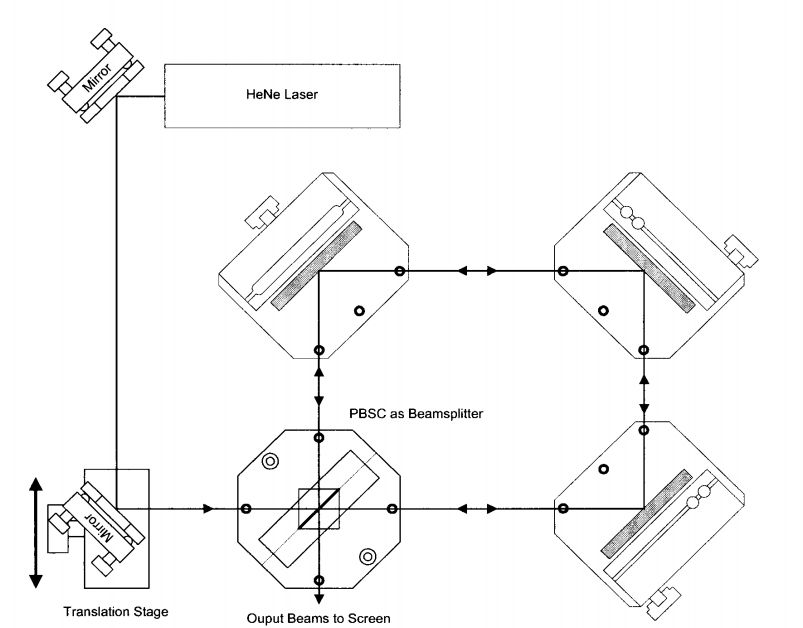
\includegraphics[width=0.6\textwidth]{pics/Aufbau.png}
  \caption{Schematische Darstellung des Sagnac-Interferometers \cite{Anleitung}.}
  \label{fig:Aufbau}
\end{figure}
\subsection{Kontrastbestimmung}
Ein Qualitätsmaß von Interferometern ist der Kontrast K. Dieser wird durch die maximalen
und minimalen Intensitäten mit :
\begin{equation}
	K= \frac{I_{\text{max}}-I_{\text{min}}}{I_{\text{max}}+I_{\text{min}}}
	\label{eq:Kontrast}
\end{equation}
bestimmt. Dabei ist 1 der bestmögliche und 0 der schlechteste Wert. \\
Die Intensität kann mit
\begin{equation}
	I \propto <|E_1 \cos{(\phi)}\cos{(\omega t)} + E_2 \sin{(\phi)}\cos{(\omega t + \delta)} |^2>
\end{equation}
beschreiben werden. Da sie sich  Dabei beschreibt $\phi$ den Polarisationswinkel, $E_0$ die
Amplituden der Wellen und $\delta$ eine Phasenverschiebung.
Für konstruktive bzw. destruktive Interferenz gilt:
\begin{align*}
	\delta_{\text{k}}&=2 n \pi , n \in \mathds{N}_0 \\
	\delta_{\text{d}}&=(2n+1)\pi , n \in \mathds{N} .
\end{align*}
Weiterhin gilt $<\cos(\omega t + \delta)>=1/2$ .
Damit lässt sich die Intensität ausdrücken zu:
\begin{equation}
	I \propto I_{\text{Laser}}\left(1\pm 2\cos{(\phi)}\sin{(\phi)}\right)
\end{equation}
Wobei die Amplituden über die Amplituden des Lasers $I_{\text{Laser}\propto (E_1+E_2)^2}$
ausgedrückt werden.
Daraus kann unter der Verwendung des Additionstheorems $\sin{(2\phi)}=2\cos{(\phi)}\sin{(\phi)}$
die Gleichung \ref{eq:Kontrast} umgeformt werden:
\begin{equation}
	K=\sin{2\phi}
	\label{eq:Kontrast2}
\end{equation}
\subsection{Brechungsindex}
Ist der Kontrast ausreichend hoch, kann über die Abzählung der Interferenz Maxima der
Brechungsindex von Proben bestimmt werden.\\
Die Anzahl der Maxima lässt sich als Funktion des Phasenversatzes ausdrücken.
\begin{equation}
	N=\frac{\delta}{2\pi}
\end{equation}
